\documentclass[11pt]{article}
\usepackage[a4paper,margin=1in]{geometry}
\usepackage{amsmath,amssymb}
\usepackage{graphicx}
\usepackage{booktabs}
\usepackage{array}
\usepackage{hyperref}
\usepackage{float}
\usepackage{xcolor}
\usepackage{listings}
\usepackage{caption}
\usepackage{subcaption}
\usepackage{enumitem}
\usepackage{microtype}

\hypersetup{colorlinks=true,linkcolor=blue!50!black,citecolor=blue!50!black,urlcolor=blue!50!black}
\newcommand{\code}[1]{\texttt{#1}}
\newcolumntype{L}[1]{>{\raggedright\arraybackslash}p{#1}}

\lstset{
  basicstyle=\ttfamily\small,
  columns=fullflexible,
  breaklines=true,
  frame=single,
  backgroundcolor=\color{gray!5}
}

\title{Speech Analysis: Identification and Detection of Voiced Consonants}
\author{VE216 Project Topic 2\\Python implementation as a MATLAB substitute}
\date{April 2026}

\begin{document}
\maketitle

\begin{abstract}
This project studies the spectrum of voiced consonants and implements automatic detection of selected consonant letters in spoken command words.  Four primary voiced consonants, /d/, /g/, /l/, and /n/, are analyzed in detail; /r/ and /j/ are included as extra voiced targets and two non-target words are grouped as an ``other'' class.  Because MATLAB is unavailable locally, the full signal-processing pipeline is implemented in Python with NumPy, SciPy, and scikit-learn.  The real audio data come from the TensorFlow mini Speech Commands data set, containing 8000 one-second utterances from eight command words.  A classical detector based on short-time spectra, MFCCs, and nearest-centroid matching is compared with an AI detector implemented as a small multilayer perceptron.  On a held-out 2000-file test set, the classical detector reaches 52.25\% consonant-class accuracy, while the AI detector reaches 76.30\%.  The experiment confirms that voiced consonants are visible in short-time spectral features, but robust detection benefits from data-driven nonlinear classification.
\end{abstract}

\section{Introduction}

The project statement asks for spectral analysis of at least four voiced consonant letters and a program that detects the presence of selected letters in spoken words.  The target is not full speech recognition; it is a smaller signal-processing task: use the spectrum of consonants to identify whether a word contains a particular voiced consonant cue.

A voiced consonant has periodic glottal excitation during articulation, so its spectrum often contains harmonic structure and low-frequency voicing energy.  However, consonants differ by manner and place of articulation.  Stops such as /d/ and /g/ contain short transient bursts after closure release, nasals such as /n/ contain low-frequency resonances and antiresonances, and liquids such as /l/ and /r/ have formant-like spectral patterns.  Therefore, the relevant representation should preserve both time localization and spectral shape.

This report follows a journal-style workflow:
\begin{enumerate}[nosep]
    \item define a real-data consonant detection problem;
    \item compute short-time spectral and cepstral features;
    \item visualize representative spectra for the target consonants;
    \item implement a classical nearest-centroid detector;
    \item implement an AI detector and compare the two methods.
\end{enumerate}

\section{Data set and problem setting}

\subsection{Real data}

The experiment uses the TensorFlow mini Speech Commands data set from the official TensorFlow audio tutorial.  It is a subset of the Speech Commands data set introduced by Warden for limited-vocabulary speech recognition.  The local data used in this project contain 8000 WAV files, sampled at 16 kHz, with 1000 examples for each of the following words:
\[
\texttt{down},\ \texttt{go},\ \texttt{left},\ \texttt{no},\ \texttt{right},\ \texttt{yes},\ \texttt{stop},\ \texttt{up}.
\]

The words are mapped to their initial consonant targets as shown in Table~\ref{tab:mapping}.  The project requires at least four letters, so /d/, /g/, /l/, and /n/ are the primary targets.  /r/ and /j/ are included as additional voiced consonantal classes.  \texttt{stop} and \texttt{up} are used as non-target examples and merged into an \code{other} class.

\begin{table}[H]
\centering
\caption{Word-to-consonant mapping used by the detector.}
\label{tab:mapping}
\begin{tabular}{@{}lll@{}}
\toprule
Word & Target class & Role \\
\midrule
\texttt{down} & /d/ & primary voiced stop \\
\texttt{go} & /g/ & primary voiced stop \\
\texttt{left} & /l/ & primary voiced liquid \\
\texttt{no} & /n/ & primary voiced nasal \\
\texttt{right} & /r/ & extra voiced liquid \\
\texttt{yes} & /j/ & extra voiced glide \\
\texttt{stop} & other & non-target initial /s/ \\
\texttt{up} & other & vowel-initial non-target \\
\bottomrule
\end{tabular}
\end{table}

This mapping is a controlled simplification.  The detector classifies the most salient initial consonant of short command words, rather than performing phone boundary segmentation inside long continuous speech.  This is still a meaningful version of the project task because the program detects whether a selected consonant cue is present in a spoken word.

\subsection{Train-test split}

The data set is split at file level into 6000 training files and 2000 held-out testing files, stratified by target class.  The split is fixed with random seed 216 for reproducibility.  The final class counts are:

\begin{center}
\begin{tabular}{@{}lrrrrrrr@{}}
\toprule
Class & /d/ & /g/ & /l/ & /n/ & /r/ & /j/ & other \\
\midrule
Files & 1000 & 1000 & 1000 & 1000 & 1000 & 1000 & 2000 \\
\bottomrule
\end{tabular}
\end{center}

\section{Signal-processing method}

\subsection{Preprocessing}

Each WAV file is converted to mono, normalized to unit peak amplitude, and padded or cropped to one second.  A pre-emphasis filter is applied:
\begin{equation}
    y[n] = x[n] - 0.97x[n-1].
\end{equation}
The signal is then divided into 25 ms Hamming-windowed frames with a 10 ms hop.  This is a standard short-time assumption: speech is nonstationary over long intervals, but approximately stationary inside a short frame.

\subsection{Short-time spectrum}

For a frame $x_m[n]$, the short-time Fourier transform is
\begin{equation}
    X_m[k] = \sum_{n=0}^{N-1} x_m[n]w[n]e^{-j2\pi kn/N}.
\end{equation}
The spectrogram uses $20\log_{10}|X_m[k]|$.  It shows how consonant energy is distributed over time and frequency.  This is especially useful for distinguishing stops, nasals, and liquids because their acoustic cues are not equally visible in a full-word average spectrum.

\subsection{MFCCs and classical spectral descriptors}

The main feature representation is a combination of MFCCs and interpretable spectral descriptors.  For each frame, the power spectrum is passed through 40 triangular mel filters.  The log mel energies are transformed by a discrete cosine transform:
\begin{equation}
    c_q = \sum_{m=1}^{M} \log E_m \cos\left[\frac{\pi q}{M}(m-0.5)\right], \qquad q=0,\ldots,12.
\end{equation}
The first 13 MFCCs are kept.  MFCCs are widely used because they summarize the spectral envelope in a way that roughly matches human auditory frequency resolution.

Additional descriptors are computed from each frame:
\begin{align}
    \text{centroid} &= \frac{\sum_k f_k |X[k]|}{\sum_k |X[k]|}, \\
    \text{bandwidth} &= \sqrt{\frac{\sum_k |X[k]|(f_k-\text{centroid})^2}{\sum_k |X[k]|}}, \\
    \text{rolloff}_{0.85} &= \min f_i \quad \text{s.t.}\quad \sum_{k\le i}|X[k]| \ge 0.85\sum_k |X[k]|.
\end{align}
RMS energy and zero-crossing rate are also included.  The final feature vector concatenates mean and standard deviation statistics with the fixed-length MFCC time sequence.  The statistical part supports interpretable comparison; the time-sequence part gives the AI model access to temporal order.

\section{Implemented detectors}

\subsection{Classical nearest-centroid detector}

The classical baseline uses the same handcrafted features but no neural network.  After standardization, each target class is represented by its training-set centroid.  A test utterance is assigned to the class with the largest cosine similarity:
\begin{equation}
    \hat{y} = \arg\max_c \frac{z^\top \mu_c}{\|z\|_2\|\mu_c\|_2},
\end{equation}
where $z$ is the standardized feature vector and $\mu_c$ is the centroid for class $c$.

\begin{lstlisting}[caption={Classical detector pseudocode.}]
for each training utterance:
    compute STFT, MFCC, spectral statistics
standardize all feature vectors
for each consonant class c:
    centroid[c] = mean(feature vectors with label c)
for each test utterance z:
    predict class with maximum cosine_similarity(z, centroid[c])
\end{lstlisting}

This detector is transparent: its decision is based on similarity to average spectral templates.  Its weakness is that it cannot easily model nonlinear speaker variation, timing variation, or overlapping cues.

\subsection{AI detector}

The AI method uses a multilayer perceptron implemented by scikit-learn.  The input feature vector is the same standardized MFCC/spectral representation.  The network has two hidden layers of 64 and 32 ReLU units and is trained by backpropagation.  It redoes the detection step with a nonlinear decision boundary:
\begin{equation}
    \hat{y}=\operatorname{softmax}(W_3\sigma(W_2\sigma(W_1z+b_1)+b_2)+b_3).
\end{equation}

This model is still small enough to explain and reproduce.  It is not a large speech-recognition system; it is an AI classifier for the same voiced-consonant detection task.

\section{Results}

\subsection{Spectral analysis}

Figure~\ref{fig:overview} shows representative waveforms and spectrograms for the four primary voiced consonants.  The stop consonants /d/ and /g/ are more transient: their cues are concentrated near the word onset and release.  The liquid /l/ and nasal /n/ show more sustained low-frequency voiced structure.  These observations justify using short-time features instead of only one global Fourier transform for the whole word.

\begin{figure}[H]
\centering
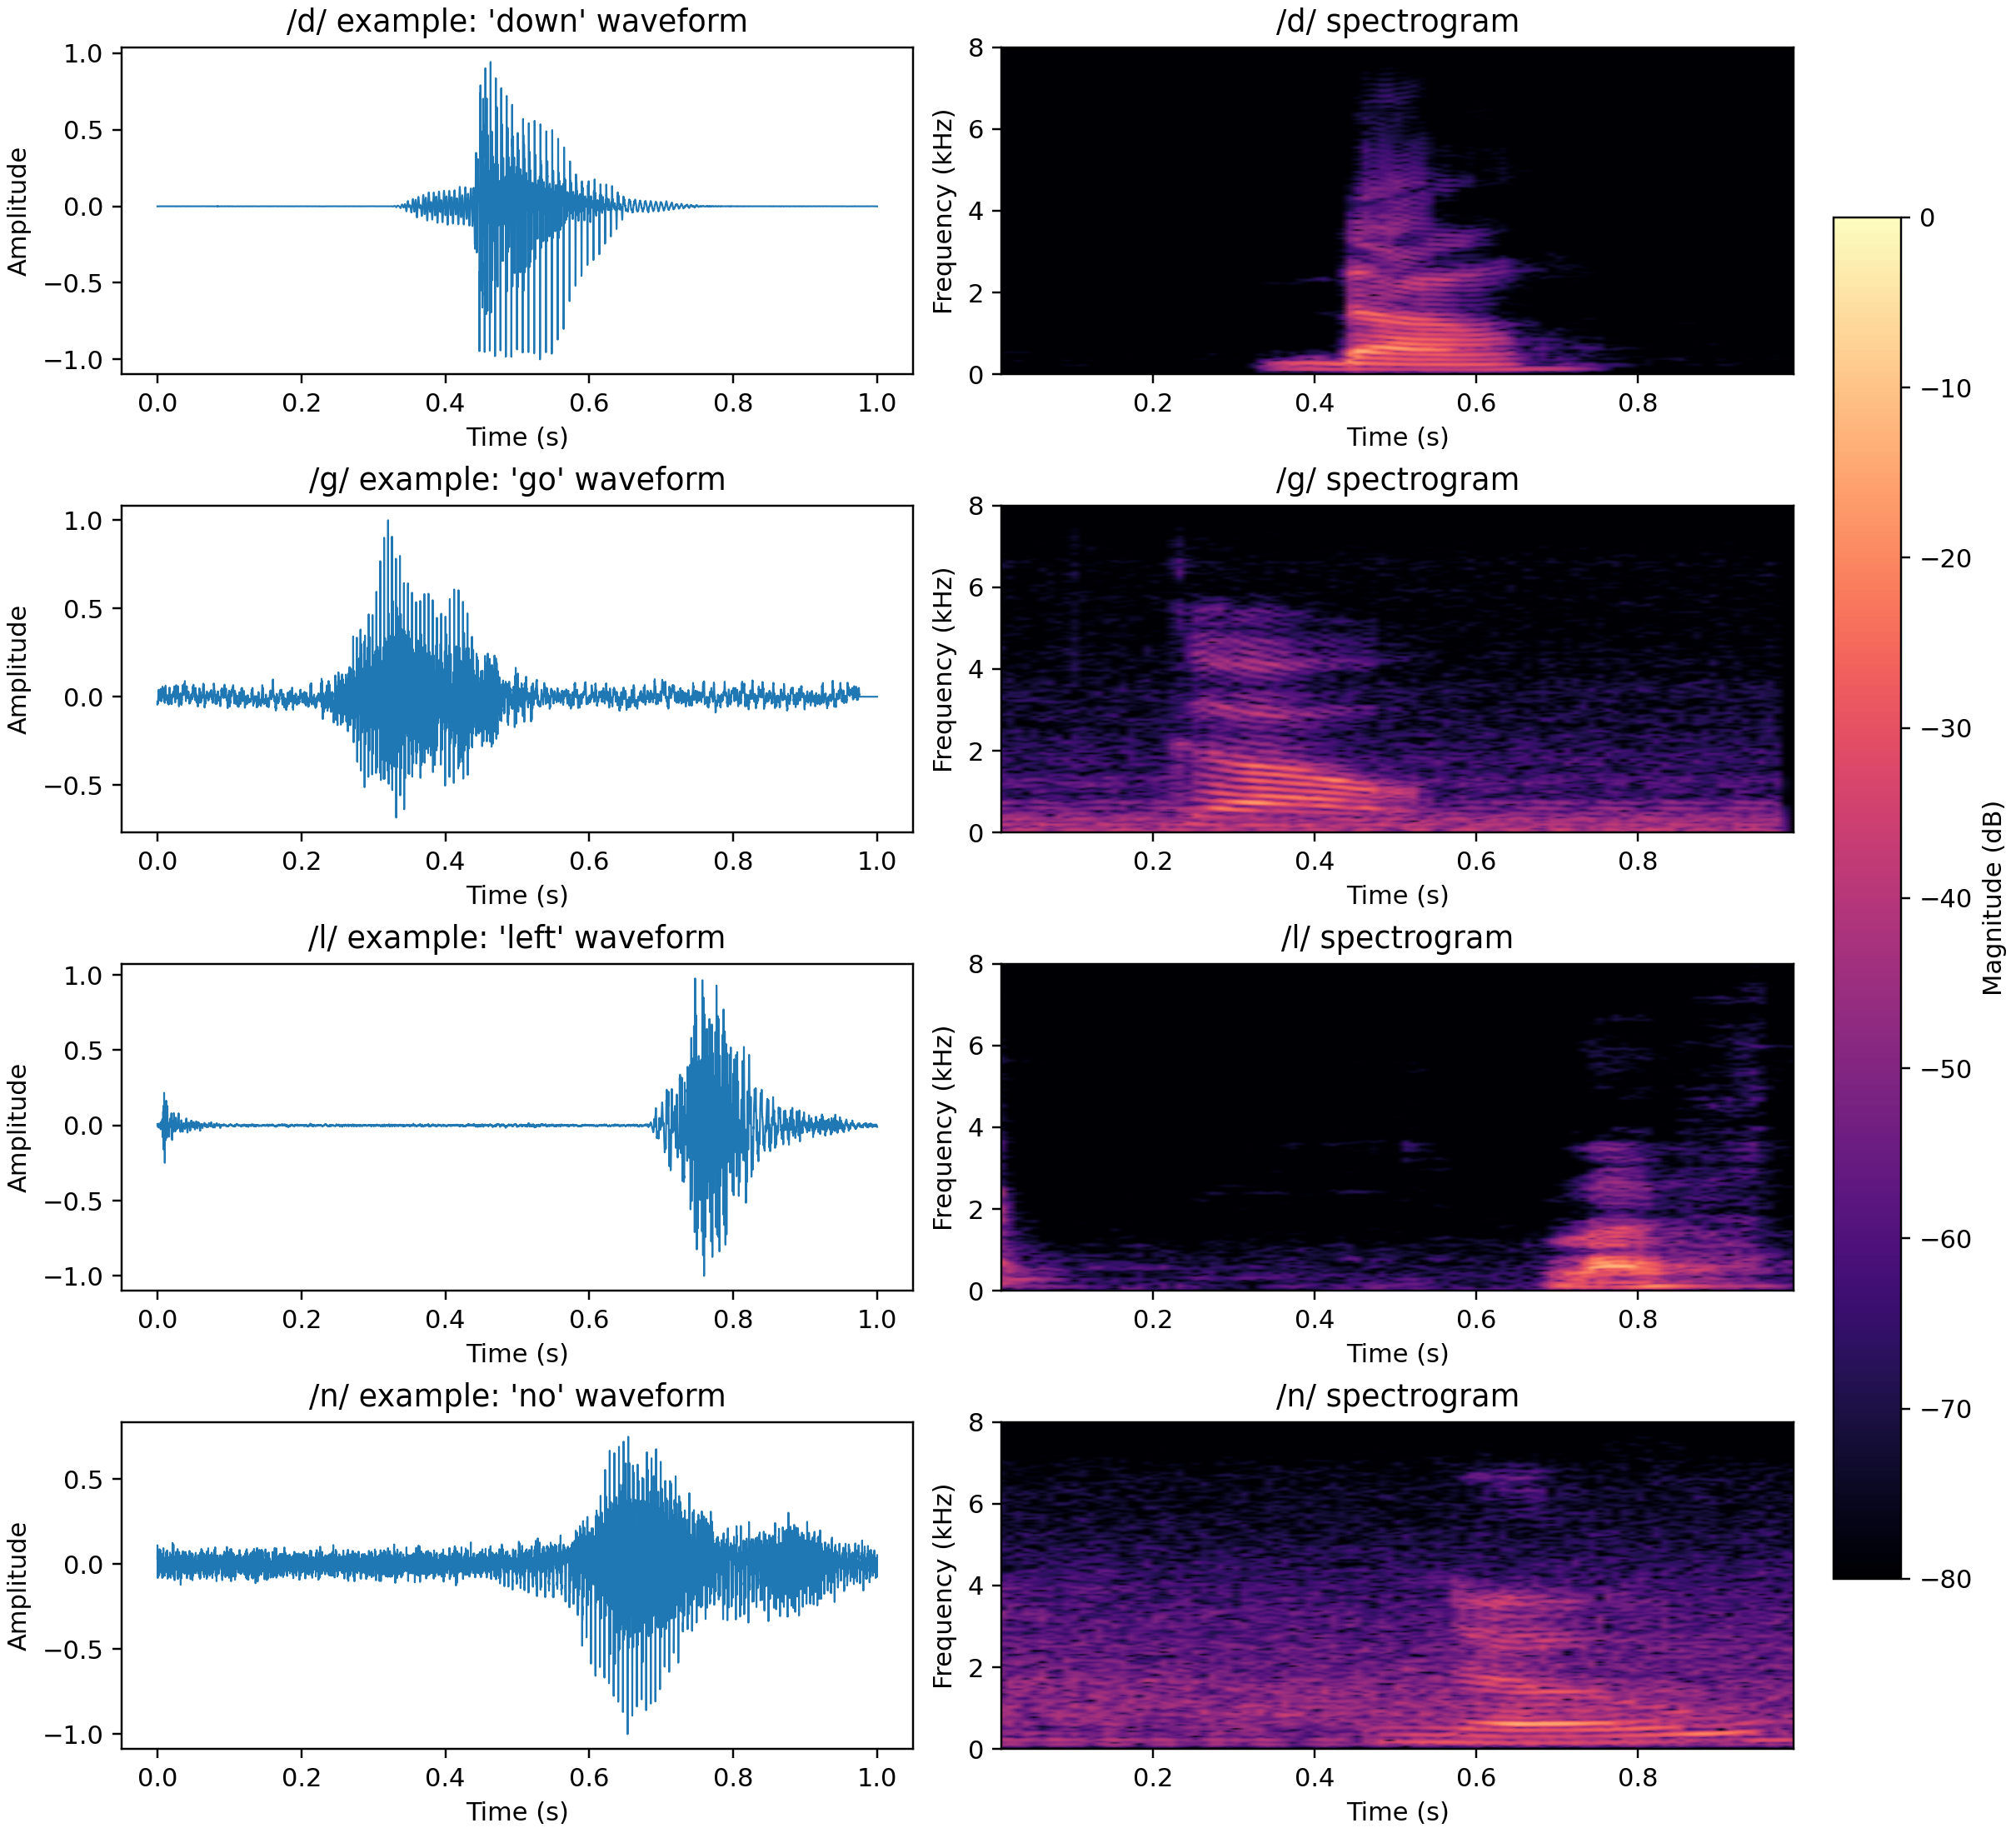
\includegraphics[width=0.98\linewidth]{figures/spectral_overview.png}
\caption{Waveforms and spectrograms for representative /d/, /g/, /l/, and /n/ examples from the real data set.}
\label{fig:overview}
\end{figure}

Figure~\ref{fig:meanspectra} compares representative short-time average spectra for all voiced target classes.  The curves are not perfectly separable by one frequency band, which explains why a simple single-threshold detector is insufficient.  The task requires a combination of spectral envelope, energy, and temporal features.

\begin{figure}[H]
\centering
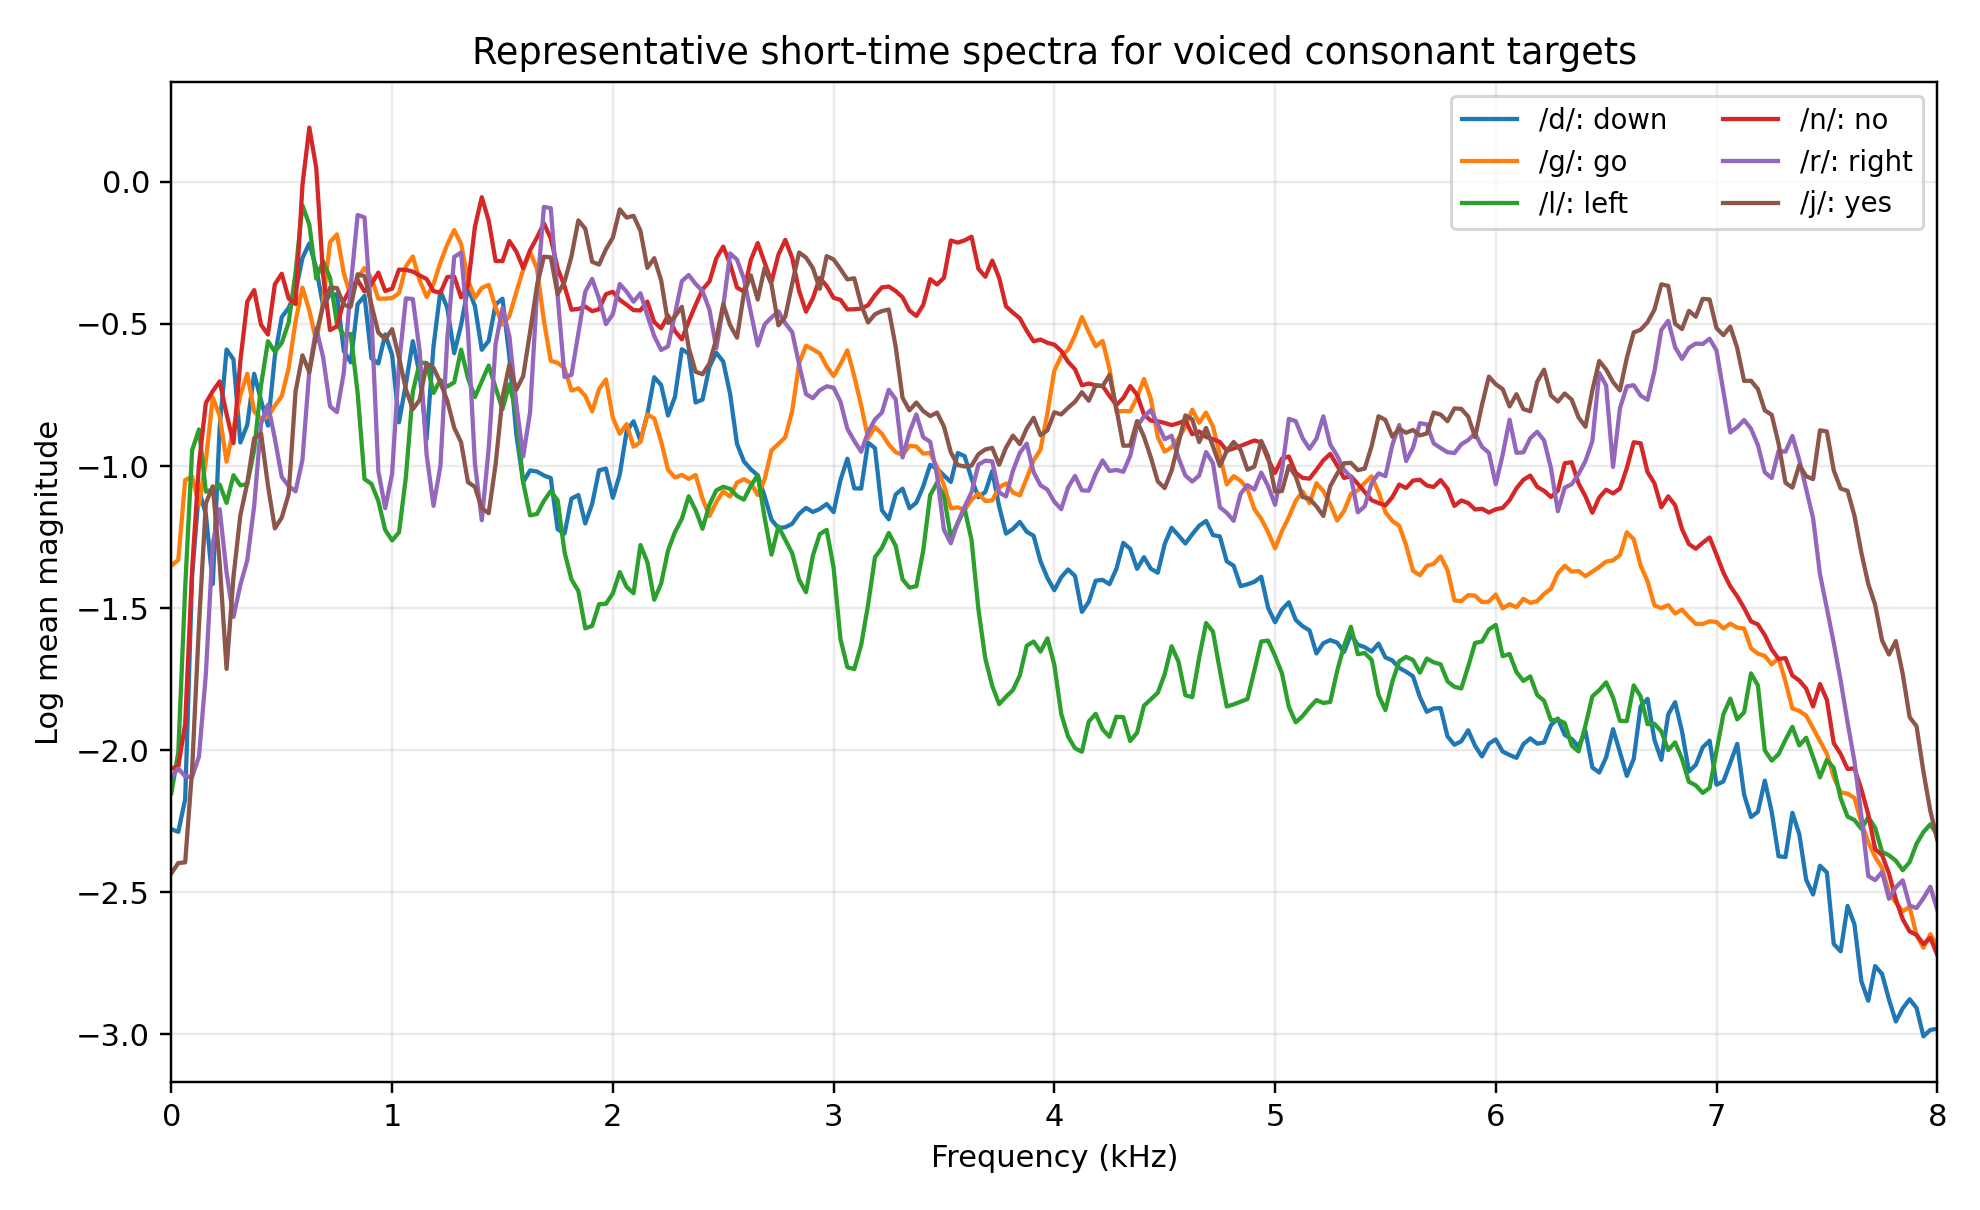
\includegraphics[width=0.82\linewidth]{figures/mean_spectra.png}
\caption{Representative short-time spectra for six voiced consonant targets.}
\label{fig:meanspectra}
\end{figure}

\subsection{Detection accuracy}

Table~\ref{tab:accuracy} summarizes held-out accuracy.  The AI detector improves accuracy by 24.05 percentage points over the classical centroid baseline.

\begin{table}[H]
\centering
\caption{Held-out consonant-class detection accuracy.}
\label{tab:accuracy}
\begin{tabular}{@{}lrr@{}}
\toprule
Method & Test files & Accuracy \\
\midrule
Classical MFCC nearest-centroid detector & 2000 & 52.25\% \\
AI detector: MLP on MFCC and spectral descriptors & 2000 & 76.30\% \\
\bottomrule
\end{tabular}
\end{table}

Figure~\ref{fig:confusions} gives normalized confusion matrices.  The classical method confuses several voiced classes because each centroid is only an average spectral template.  The AI method is substantially stronger, especially for /d/, /r/, /j/, and the non-target class.  The hardest primary class remains /n/, which is often confused with other voiced sonorants or with the broad \code{other} class.

\begin{figure}[H]
\centering
\begin{subfigure}{0.48\linewidth}
    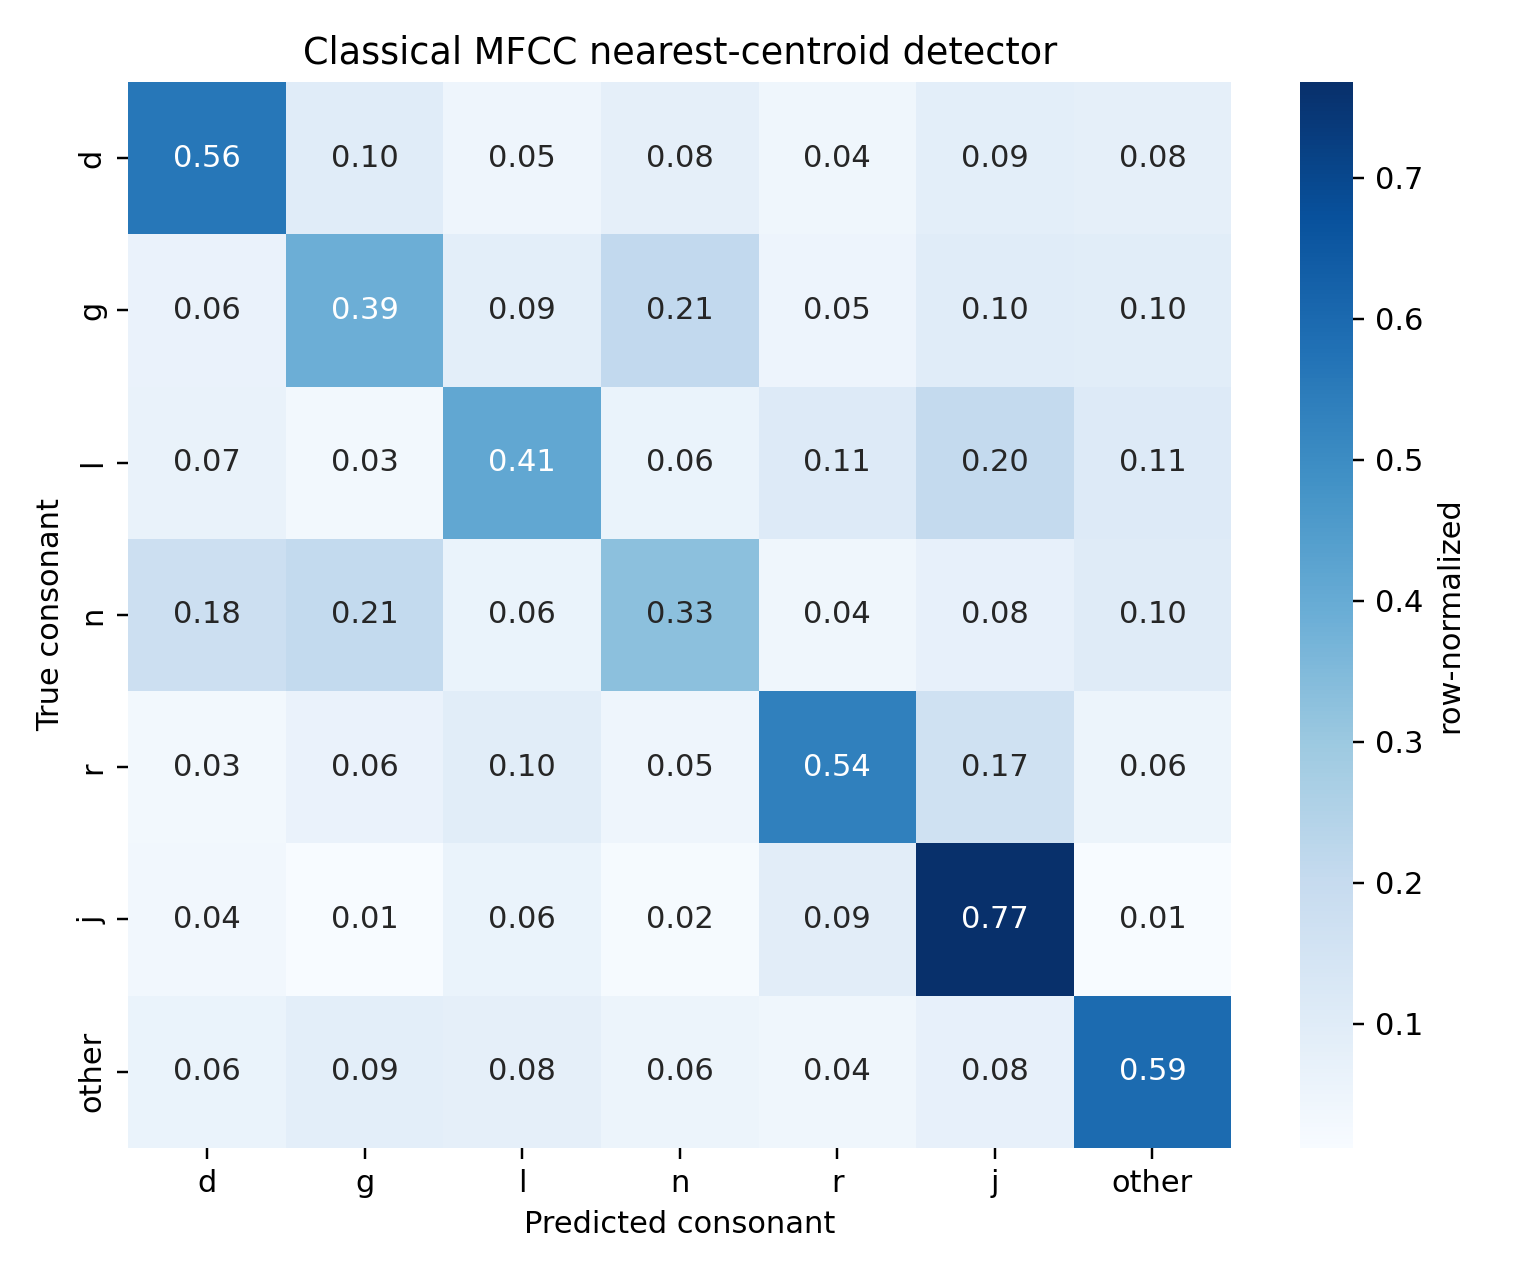
\includegraphics[width=\linewidth]{figures/confusion_centroid.png}
    \caption{Classical detector}
\end{subfigure}
\hfill
\begin{subfigure}{0.48\linewidth}
    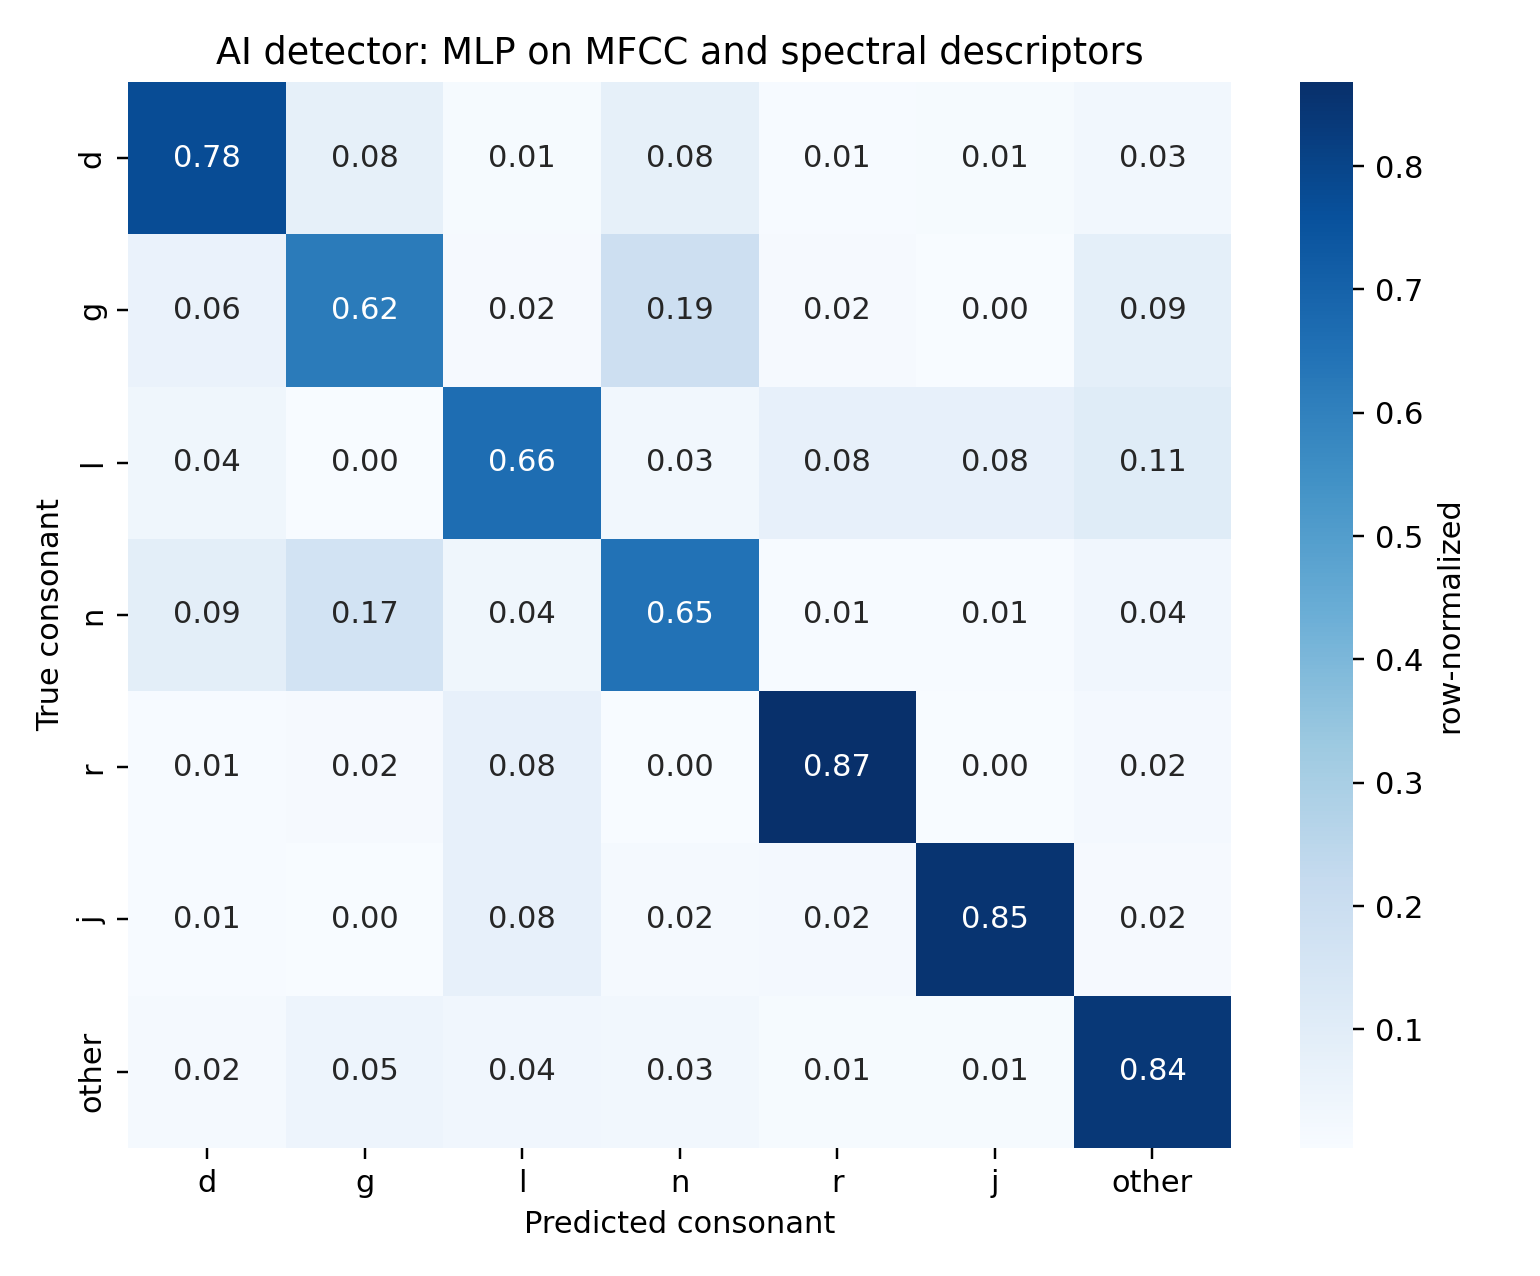
\includegraphics[width=\linewidth]{figures/confusion_mlp.png}
    \caption{AI detector}
\end{subfigure}
\caption{Row-normalized confusion matrices on the 2000-file test set.}
\label{fig:confusions}
\end{figure}

\subsection{Binary detection of the four required letters}

The project statement asks for detecting the presence of certain letters.  Table~\ref{tab:binary} reports one-vs-rest metrics for the four required voiced consonants.  The AI detector improves all four F1 scores.

\begin{table}[H]
\centering
\caption{One-vs-rest detection metrics for the four primary voiced consonants.}
\label{tab:binary}
\begin{tabular}{@{}llrrr@{}}
\toprule
Target & Method & Precision & Recall & F1 \\
\midrule
/d/ & Classical & 0.526 & 0.560 & 0.543 \\
/d/ & AI MLP & 0.755 & 0.776 & 0.765 \\
/g/ & Classical & 0.396 & 0.388 & 0.392 \\
/g/ & AI MLP & 0.628 & 0.620 & 0.624 \\
/l/ & Classical & 0.446 & 0.412 & 0.428 \\
/l/ & AI MLP & 0.695 & 0.664 & 0.679 \\
/n/ & Classical & 0.381 & 0.328 & 0.353 \\
/n/ & AI MLP & 0.623 & 0.648 & 0.635 \\
\bottomrule
\end{tabular}
\end{table}

\section{Discussion}

\subsection{What the classical method captures}

The classical method uses exactly the kind of spectrum-based reasoning expected in a signals-and-systems project.  STFT localizes consonant cues in time, MFCCs describe the spectral envelope, and centroid/bandwidth/rolloff summarize frequency distribution.  These features are interpretable and can be inspected directly from figures.

The main limitation is that a single centroid per consonant cannot represent all speakers, accents, microphone conditions, and timing differences.  For example, the /g/ in \texttt{go} may vary strongly by speaker and vowel transition, and the /n/ in \texttt{no} is influenced by the following vowel.  This reduces the effectiveness of pure template matching.

\subsection{What the AI method improves}

The MLP uses the same physical features but learns nonlinear combinations of them.  This is why it outperforms the nearest-centroid detector.  The result does not mean that AI replaces signal processing.  In this experiment, AI works because the signal-processing front end provides a compact representation: normalization, framing, STFT, mel filtering, and MFCC extraction still define the information that the model sees.

\subsection{Limitations}

This project is intentionally scoped to be reproducible within the VE216 deadline.  It has three limitations:
\begin{enumerate}[nosep]
    \item The labels are word-level initial consonant labels, not manually segmented phone labels.
    \item The data set contains command words, not arbitrary words such as \texttt{book} or \texttt{boy}.
    \item The AI model is a small classifier, not a full automatic speech recognition model.
\end{enumerate}
These limitations can be removed in future work by using a phonetically aligned corpus such as TIMIT or by manually segmenting consonant intervals in recorded words.

\section{Conclusion}

The project implemented a complete voiced-consonant analysis and detection pipeline with real speech data.  Four required voiced consonants, /d/, /g/, /l/, and /n/, were analyzed with waveforms, spectrograms, and short-time spectra.  A classical MFCC nearest-centroid detector and a small AI detector were implemented and compared.  The AI detector achieved 76.30\% test accuracy, compared with 52.25\% for the classical detector, and improved one-vs-rest F1 scores for all four required consonants.  The main conclusion is that spectral analysis provides the necessary acoustic representation, while data-driven classification improves robustness under speaker and recording variability.

\section*{Reproducibility}

The implementation files are organized as follows:
\begin{itemize}[nosep]
    \item \path{src/download_data.sh}: downloads the real audio data set.
    \item \path{src/run_experiment.py}: extracts features, trains detectors, saves metrics, and generates figures.
    \item \path{build/results/summary.json}: final test accuracy and data counts.
    \item \path{build/results/binary_detection_metrics.csv}: one-vs-rest metrics for /d/, /g/, /l/, and /n/.
    \item \path{figures/}: generated figures included in this report.
\end{itemize}

The main commands are:
\begin{lstlisting}
python -m venv .venv
.venv/bin/python -m pip install -r requirements.txt
src/download_data.sh
.venv/bin/python src/run_experiment.py
latexmk -xelatex -interaction=nonstopmode -halt-on-error report.tex
\end{lstlisting}

\begin{thebibliography}{9}

\bibitem{warden2018}
P. Warden, ``Speech Commands: A Dataset for Limited-Vocabulary Speech Recognition,'' arXiv:1804.03209, 2018. [Online]. Available: \url{https://arxiv.org/abs/1804.03209}

\bibitem{tensorflowaudio}
TensorFlow, ``Simple audio recognition: Recognizing keywords,'' official tutorial. [Online]. Available: \url{https://www.tensorflow.org/tutorials/audio/simple_audio}

\bibitem{davismermelstein1980}
S. B. Davis and P. Mermelstein, ``Comparison of parametric representations for monosyllabic word recognition in continuously spoken sentences,'' \emph{IEEE Transactions on Acoustics, Speech, and Signal Processing}, vol. 28, no. 4, pp. 357--366, 1980. doi: \href{https://doi.org/10.1109/TASSP.1980.1163420}{10.1109/TASSP.1980.1163420}.

\bibitem{scipystft}
SciPy Developers, ``scipy.signal.stft,'' SciPy documentation. [Online]. Available: \url{https://docs.scipy.org/doc/scipy/reference/generated/scipy.signal.stft.html}

\bibitem{sklearnmlp}
scikit-learn Developers, ``sklearn.neural\_network.MLPClassifier,'' scikit-learn documentation. [Online]. Available: \url{https://scikit-learn.org/stable/modules/generated/sklearn.neural_network.MLPClassifier.html}

\bibitem{librosa}
B. McFee et al., ``librosa: Audio and Music Signal Analysis in Python,'' 2015. [Online]. Available: \url{https://librosa.org/doc/latest/feature.html}

\end{thebibliography}

\end{document}
